\documentclass[12pt,letterpaper,oneside]{book}
\usepackage{../afitStyleFiles/afitThesis}
\usepackage{../afitStyleFiles/sf298}
\usepackage[pdftex,pdfpagelabels,bookmarks,hyperindex,hyperfigures]{hyperref}
\hypersetup{
    colorlinks,
    citecolor=black,
    filecolor=black,
    linkcolor=black,
    urlcolor=black
}
\usepackage{float}
\usepackage{tikz}
\usetikzlibrary{positioning}
\usepackage[percent]{overpic}

\mathchardef\mhyphen="2D % Define a "math hyphen"
\graphicspath{{../Figures/}}

\input{Preamble/titlepage}
%% myFigures.tex
% A common file to store all figure definitions
%
% In preparing your thesis, one of the first things you should do is
% organize your figures.  Then, one of the last things you'll do is
% reorder your figures so they display where you want them to in the
% text.  Organizing figure definitions in a common files helps:
%
%   1. Write new figures using earlier examples.
%
%   2.  Isolate code and minimize the risk of introducing bugs in the
%   final editing process.  Trust me, moving around just one line of
%   code is easier.
%
%   3.  Reuse figures in other papers.  <=== the best reason!
%
% Note command names can not include numbers and special characters.
%
% To make the file more searchable, use naming conventions that map
% the graphics filename labSetup.jpg to the command name \figlabSetup to the
% figure label fig:labSetup.
% 

\newcommand{\figproactiveFaultManagement}{\begin{figure}[H]
 \begin{center}
    \includegraphics[width=6in]{proactiveFaultManagement}
     \caption[Proactive Fault Management~\cite{salfnerSurvey}]{The stages of
     proactive fault management.~\cite{salfnerSurvey}.}
     \label{fig:proactiveFaultManagement}
 \end{center}
\end{figure}
}

\newcommand{\figonlinePrediction}{\begin{figure}[H]
 \begin{center}
    \includegraphics[width=6in]{onlinePrediction}
     \caption[Online Failure Prediction~\cite{salfnerSurvey}]{The timeline for OFP~\cite{salfnerSurvey}.}
     \label{fig:onlinePrediction}
 \end{center}
\end{figure}
}

\newcommand{\figfailureFlowDiagram}{\begin{figure}[H]
 \begin{center}
    \includegraphics[width=6in]{failureFlowDiagram}
     \caption[Failure Flow Diagram~\cite{salfnerSurvey}]{How faults and errors evolve into failure with the associated methods for detection represented by enclosing gray boxes~\cite{salfnerSurvey}.}
     \label{fig:failureFlowDiagram}
 \end{center}
 %\vspace{-0.2 in}
\end{figure}
}

\newcommand{\figROC}{\begin{figure}[H]
 \begin{center}
    \includegraphics[width=3in]{ROC}
     \caption[Sample ROC Plots~\cite{salfnerSurvey}]{ROC plots of perfect, average, and random predictors~\cite{salfnerSurvey}.}
     \label{fig:ROC}
 \end{center}
\end{figure}
}

\newcommand{\figprecisionRecallCurve}{\begin{figure}[H]
 \begin{center}
    \includegraphics[width=3in]{precisionRecallCurve}
     \caption[Sample Precision/Recall Curves~\cite{salfnerSurvey}]{Sample precision/recall curves~\cite{salfnerSurvey}.  Curve $A$ represents a poorly performing predictor, curve $B$ represents an average predictor, and curve $C$ represents an exceptional predictor.}
     \label{fig:precisionRecallCurve}
 \end{center}
\end{figure}
}

\newcommand{\figpatternRecognition}{\begin{figure}[H]
 \begin{center}
    \includegraphics[width=6in]{patternRecognition}
     \caption[Pattern recognition in reported errors~\cite{salfnerSurvey}]{How pattern recognition is accomplished in reported errors~\cite{salfnerSurvey}.}
     \label{fig:patternRecognition}
 \end{center}
\end{figure}
}

\newcommand{\figAFP}{\begin{figure}[H]
 \begin{center}
    \includegraphics[width=5in]{AFP}
     \caption[AFP Framework Implementation~\cite{irrera2015}]{How the AFP framework is implemented~\cite{irrera2015}.}
     \label{fig:AFP}
 \end{center}
\end{figure}
}

\definecolor{airforceblue}{rgb}{0.36, 0.54, 0.66}
\definecolor{armygreen}{rgb}{0.29, 0.33, 0.13}

\newcommand{\figannotatedAFP}{\begin{figure}[ht!]
 \begin{center}
     \begin{overpic}[width=5in,scale=.25]{annotatedAFP}
       \put(8,0){
         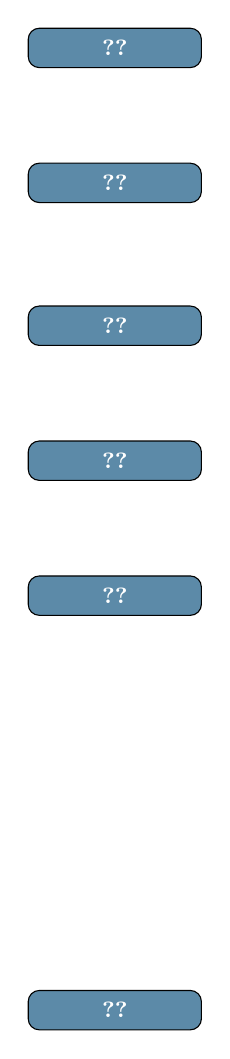
\begin{tikzpicture}
           [node font=\footnotesize, label/.style={rectangle, draw,
           fill=airforceblue, text width=2cm, text badly centered, minimum
           height=0.5cm, rounded corners}]

           \node[label] (FPMgr)
             {\textcolor{white}{\ref{sec:failurePrediction}}};
           \node[label, below=1.2cm of FPMgr] (FIMgr) 
             {\textcolor{white}{\ref{sec:faultInjectionMgr}}};
           \node[label, below=1.3cm of FIMgr] (WMgr) 
             {\textcolor{white}{\ref{sec:workloadMgr}}};
           \node[label, below=1.2cm of WMgr] (EMMgr) 
             {\textcolor{white}{\ref{sec:eventsManagerMgr}}};
           \node[label, below=1.2cm of EMMgr] (SMgr) 
             {\textcolor{white}{\ref{sec:sandboxMgr}}};
           \node[label, below=4.75cm of SMgr] (Controller) 
             {\textcolor{white}{\ref{sec:controller}}};
         \end{tikzpicture}
       }

       \put(40,60.5){
         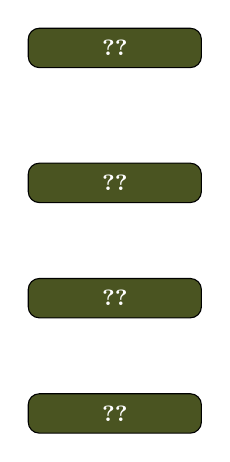
\begin{tikzpicture}
           [node font=\footnotesize, label/.style={rectangle, draw,
           fill=armygreen, text width=2cm, text badly centered, minimum
           height=0.5cm, rounded corners}]

           \node[label] (Sandbox)
             {\textcolor{white}{\ref{sec:sandbox}}};
           \node[label, below=1.2cm of Sandbox] (SBFITool)
             {\textcolor{white}{\ref{sec:faultInjectionTool}}};
           \node[label, below=0.95cm of SBFITool] (SBMTool) 
             {\textcolor{white}{\ref{sec:sandboxMonitoringTool}}};
           \node[label, below=0.95cm of SBMTool] (SBWorkload) 
             {\textcolor{white}{\ref{sec:sandboxWorkload}}};
         \end{tikzpicture}
       }

       \put(66,0){
         
\begin{tikzpicture}
           [node font=\footnotesize, label/.style={rectangle, draw,
           fill=armygreen, text width=2cm, text badly centered, minimum
           height=0.5cm, rounded corners}]

           \node[label] (MonTool)
             {\textcolor{white}{\ref{sec:targetMonitoringTool}}};
           \node[label, below=7.85cm of MonTool] (Target)
             {\textcolor{white}{\ref{sec:target}}};
         \end{tikzpicture}
       }
     \end{overpic}
     \caption[Annotated AFP Framework~\cite{irrera2015}]{The AFP framework
     implementation~\cite{irrera2015} with modified components highlighted.}
     \label{fig:annotatedAFP}
 \end{center}
\end{figure}
}

\newcommand{\figTrainingPhase}{\begin{figure}[H]
 \begin{center}
  \includegraphics[width=4in]{TrainingPhase}
  \caption[AFP Training Phase~\cite{irrera2015}]{The flow of the major steps
    involved in the AFP framework training phase~\cite{irrera2015}.}
  \label{fig:TrainingPhase}
 \end{center}
\end{figure}
}

\newcommand{\figExecutionPhase}{\begin{figure}[!ht]
  \begin{center}
    \includegraphics[width=2.5in]{ExecutionPhase}
    \caption[AFP Execution Phase~\cite{irrera2015}]{The flow of the major steps
    involved in the AFP framework execution phase~\cite{irrera2015}.}
    \label{fig:ExecutionPhase}
  \end{center}
\end{figure}
}

\newcommand{\figAuthDCPPS}{\begin{figure}[ht!]
 \begin{center}
  \includegraphics[width=4in]{authDCPPS}
  \caption[Domain Controller Packets per Second]{How many packets per second
  were sent or received by the domain controller across all five rounds of the
  first test.  In each test, we captured approximately 1.8 million packets.}
  \label{fig:authDCPPS}
 \end{center}
\end{figure}
}

\newcommand{\figAuthClientPPS}{\begin{figure}[ht!]
 \begin{center}
  \includegraphics[width=4in]{authClientPPS}
  \caption[Client Packets per Second]{How many packets per second were sent or
  received by one of the clients across all five rounds of the first test.}
  \label{fig:authClientPPS}
 \end{center}
\end{figure}
}

\newcommand{\figAuthDCMetrics}{\begin{figure}[ht!]
 \begin{center}
  \includegraphics[width=4in]{authDCMetrics}
  \caption[Test 1:  Domain Controller Metrics]{Domain controller CPU and memory
  utilization during the first test.}
  \label{fig:authDCMetrics}
 \end{center}
\end{figure}
}



\newcommand{\tabFaults}{
\begin{table}[!ht]
  \centering
  \caption[Fault Operators Injected~\cite{gswfit}]{Fault operators used for
  fault injection~\cite{gswfit}.}\label{tab:faults}
\begin{tabulary}{\textwidth}{ | c | l | C | } 
\hline
  \textbf{Type}  & \textbf{Description}  & \textbf{\ac{ODC} Classes}  \\ \hline \hline
  MIFS & Missing ``If (cond) \{ statement(s) \}''          & Algorithm  \\ \hline
  MFC  & Missing function call                             & Algorithm  \\ \hline
  MLAC & Missing ``AND EXPR'' in expression used as branch & Checking   \\ \hline
  MLPA & Missing small and localized part of the algorithm & Algorithm  \\ \hline
  WVAV & Wrong value assigned to a value                   & Assignment \\ \hline
  MVI  & Missing variable initialization                   & Assignment \\ \hline
  MVAV & Missing variable assignment using a value         & Assignment \\ \hline
  WPFV & Wrong variable used in parameter of function call & Interface  \\ \hline
\end{tabulary}
\end{table}
}

\newcommand{\tabTranslationThirtyTwo}{
\begin{table}[htbp]
  \centering
  \caption[Funtion Entry/Exit Patterns (IA32)~\cite{gswfit}]{Function
  entry/exit patterns in IA32 bytecode~\cite{gswfit}.}
  \label{tab:translationThirtyTwo}
\begin{tabular}{ | l | l | l | l | }
\hline
  \multicolumn{2}{|c|}{\textbf{Module Entry Point}}& 
  \multicolumn{2}{c|}{\textbf{Module Exit Point}} \\ \hline

  \textbf{Instruction} & \textbf{Explanation} &
  \textbf{Instruction} & \textbf{Explanation} \\ \hline \hline

  push ebp & stack frame & move esp,ebp & stack frame \\ \hline
  mov ebp, esp & setup & pop ebp & cleanup \\ \hline
  sub esp, \emph{immed} &  & ret &  \\ \hline
\end{tabular}
\end{table}
}

\newcommand{\tabTranslationSixtyFour}{
\begin{table}[htbp]
  \centering
  \caption[Funtion Entry/Exit Patterns (x86-64)~\cite{gswfit}]{Function
  entry/exit patterns in x86-64 bytecode~\cite{gswfit}.}
  \label{tab:translationSixtyFour}
\begin{tabular}{ | l | l | l | l | }
\hline
  \multicolumn{2}{|c|}{\textbf{Module Entry Point}}& 
  \multicolumn{2}{c|}{\textbf{Module Exit Point}} \\ \hline

  \textbf{Instruction} & \textbf{Explanation} & 
  \textbf{Instruction} & \textbf{Explanation} \\ \hline \hline

  push rbp & stack frame & add rsp, \emph{immed} & stack frame \\ \hline
  sub rsp, \emph{immed} &  & pop rbp & cleanup \\ \hline
  mov rbp, rdx & setup & ret &  \\ \hline
\end{tabular}
\end{table}
}

\newcommand{\tabHypervisorOne}{
\begin{table}[htbp]
  \centering
  \caption[Hypervisor 1 (Sandbox/Target)]{Hypervisor 1 configuration
  (sandbox/target).} \label{tab:hyp1}
  \begin{tabular}{ | c | l | l | c | l |}
    \hline
    Qty. & Role   & Operating System    & CPU / Mem. \\ \hline\hline
    1    & DC     & Win. Server 2008 R2 & 2 / 2 GB   \\ \hline
    1    & Web    & Win. Server 2008 R2 & 2 / 2 GB   \\ \hline
    5    & Client & Win. 7              & 1 / 512 MB \\ 
    \hline
  \end{tabular}
\end{table}
}


\newcommand{\tabHypervisorTwo}{
\begin{table}[htbp]
  \centering
  \caption[Hypervisor 2 (Controller)]{Hypervisor 2 configuration (controller).}
  \label{tab:hyp2}
  \begin{tabular}{ | c | l | l | c | l |}
    \hline
    Qty. & Role & Operating System    & CPU / Mem. \\ \hline\hline
    1    & RDP  & Win. Server 2008 R2 & 1 / 4 GB   \\ \hline
    1    & Log  & Ubuntu 14.04 LTS    & 1 / 1 GB   \\ 
    \hline
  \end{tabular}
\end{table}
}

\newcommand{\tabMessage}{
\begin{table}[!ht] \centering
  \caption[Example MSWinEventLog Authentication Message]{Typical authentication
  message sent as keys that correspond to the values as designated in the
  \emph{Snare} protocol for MSWinEventLog used by the SolarWinds syslog agent.}
  \label{tab:message}
  \begin{tabular}{ | l | l | }
    \hline
      Key                 & Value                               \\ \hline\hline
      HostName            & dc.afnet.com                        \\ \hline
      Criticality         & 5                                   \\ \hline
      EventLogSource      & Security                            \\ \hline
      Counter             & 3                                   \\ \hline
      SubmitTime          & Sun May 08 14:31:50 2016            \\ \hline
      EventID             & 4672                                \\ \hline
      SourceName          & Microsoft-Windows-Security-Auditing \\ \hline
      UserName            & N/A                                 \\ \hline
      SIDType             & Audit Success                       \\ \hline
      EventLogType        & dc.afnet.com                        \\ \hline
      ComputerName        & 12548                               \\ \hline
      CategoryString      & Special privileges assigned to\dots \\ \hline
      ExtendedDataString  & Security ID:  S-1-5-21-2379403\dots \\ 
    \hline
  \end{tabular}
\end{table}
}

\newcommand{\tabSlidingWindow}{
\begin{table}[!ht] \centering
  \caption[Sample Data Window Translation]{Sample message data window after
  translation.} \label{tab:window}
  \begin{tabular}{ | l | l | }
    \hline
      Predictor                   & Value \\ \hline\hline
      FailureWindow               & 0     \\ \hline
      NumObservations             & 2     \\ \hline
      Criticality: 6              & 2     \\ \hline
      Criticality: 2              & 0     \\ \hline
      Criticality: 4              & 0     \\ \hline
      EventLogSource: Application & 1     \\ \hline
      EventLogSource: System      & 1     \\ 
    \hline
  \end{tabular}
\end{table}
}

\newcommand{\tabMemLeakPreUpdateSVMStats}{
\begin{table}[!t] \centering
  \caption[Pre-Update, Memory Leak, \ac{SVM} Statistics]{Classification
  statistics on test data created before software updates.}
  \label{tab:memLeakPreUpdateSVMStats}
  \begin{tabular}{ | l | l | }
    \hline
      Statistic           & Value  \\ \hline\hline
      True Positive Rate  & 0.8525 \\ \hline
      False Positive Rate & 0.0098 \\ \hline
      Accuracy            & 0.9777 \\ \hline
      Precision           & 0.8966 \\ \hline
      Recall              & 0.8525 \\ \hline
      F-Measure           & 0.8739 \\
    \hline
  \end{tabular}
\end{table}
}
%%%%%%%%%%%%%%%%%%%%%%%%%%%%%%%%%%%%%%%%%%%%%%%%%%%%%%%%%%%%%%%%%%%%%%%%%%%%%%%
%%%%   SVM   %%%%
% Pre-Update
\newcommand{\tabMemLeakPreUpdateSVMConfusionMatrix}{
  \begin{table}[!ht]
    \centering
    \caption[Pre-Update, Memory Leak, \ac{SVM} Confusion Matrix]{Confusion matrix
    on test data created before software updates on threshold with highest
    F-Measure (0.8739) using \ac{SVM}.}
    \label{tab:memLeakPreUpdateSVMConfusionMatrix}
    \begin{tabular}{llll}
                                                               &                                       & \multicolumn{2}{c}{\textbf{Actual}}                                        \\ \cline{3-4} 
                                                               & \multicolumn{1}{l|}{}                 & \multicolumn{1}{l|}{\textbf{Fail}} & \multicolumn{1}{l|}{\textbf{No-Fail}} \\ \cline{2-4} 
      \multicolumn{1}{c|}{\multirow{2}{*}{\textbf{Predicted}}} & \multicolumn{1}{l|}{\textbf{Fail}}    & \multicolumn{1}{l|}{52}            & \multicolumn{1}{l|}{6}                \\ \cline{2-4} 
      \multicolumn{1}{c|}{}                                    & \multicolumn{1}{l|}{\textbf{No-Fail}} & \multicolumn{1}{l|}{9}             & \multicolumn{1}{l|}{607}              \\ \cline{2-4} 
    \end{tabular}
  \end{table}
}

% Post-Update (old model)

% Post-Update New Model

%%%%   BOOSTING   %%%%
% Pre-Update
\newcommand{\tabMemLeakPreUpdateBoostingConfusionMatrix}{
  \begin{table}[!ht]
    \centering
    \caption[Pre-Update, Memory Leak, Boosting Confusion Matrix]{Confusion
    matrix on test data created before software updates on threshold with
    highest F-Measure (0.9917) using boosting.}
    \label{tab:memLeakPreUpdateBoostingConfusionMatrix}
    \begin{tabular}{llll}
                                                               &                                       & \multicolumn{2}{c}{\textbf{Actual}}                                        \\ \cline{3-4} 
                                                               & \multicolumn{1}{l|}{}                 & \multicolumn{1}{l|}{\textbf{Fail}} & \multicolumn{1}{l|}{\textbf{No-Fail}} \\ \cline{2-4} 
      \multicolumn{1}{c|}{\multirow{2}{*}{\textbf{Predicted}}} & \multicolumn{1}{l|}{\textbf{Fail}}    & \multicolumn{1}{l|}{60}            & \multicolumn{1}{l|}{0}                \\ \cline{2-4} 
      \multicolumn{1}{c|}{}                                    & \multicolumn{1}{l|}{\textbf{No-Fail}} & \multicolumn{1}{l|}{1}             & \multicolumn{1}{l|}{412}              \\ \cline{2-4} 
    \end{tabular}
  \end{table}
}

% Post-Update (old model)
\newcommand{\tabMemLeakPostUpdateBoostingSameModelConfusionMatrix}{
  \begin{table}[!ht]
    \centering
    \caption[Post-Update, Memory Leak, Same Model, Confusion
    Matrix]{Post-update failure data confusion matrix on threshold with
    highest F-Measure (0.4691) using model trained on failure data generated
    before software update.}
    \label{tab:memLeakPostUpdateBoostingSameModelConfusionMatrix}
    \begin{tabular}{llll}
                                                               &                                       & \multicolumn{2}{c}{\textbf{Actual}}                                        \\ \cline{3-4} 
                                                               & \multicolumn{1}{l|}{}                 & \multicolumn{1}{l|}{\textbf{Fail}} & \multicolumn{1}{l|}{\textbf{No-Fail}} \\ \cline{2-4} 
      \multicolumn{1}{c|}{\multirow{2}{*}{\textbf{Predicted}}} & \multicolumn{1}{l|}{\textbf{Fail}}    & \multicolumn{1}{l|}{19}            & \multicolumn{1}{l|}{1}                \\ \cline{2-4} 
      \multicolumn{1}{c|}{}                                    & \multicolumn{1}{l|}{\textbf{No-Fail}} & \multicolumn{1}{l|}{42}            & \multicolumn{1}{l|}{222}              \\ \cline{2-4} 
    \end{tabular}
  \end{table}
}

% Post-Update New Model
\newcommand{\tabMemLeakPostUpdateBoostingConfusionMatrix}{
  \begin{table}[!ht]
    \centering
    \caption[Post-Update, Memory Leak, New Model, Confusion
    Matrix]{Post-update failure data confusion matrix on threshold with
    highest F-Measure (0.9355) using model trained on failure data generated
    after software update.}
    \label{tab:memLeakPostUpdateBoostingConfusionMatrix}
    \begin{tabular}{llll}
                                                               &                                       & \multicolumn{2}{c}{\textbf{Actual}}                                        \\ \cline{3-4} 
                                                               & \multicolumn{1}{l|}{}                 & \multicolumn{1}{l|}{\textbf{Fail}} & \multicolumn{1}{l|}{\textbf{No-Fail}} \\ \cline{2-4} 
      \multicolumn{1}{c|}{\multirow{2}{*}{\textbf{Predicted}}} & \multicolumn{1}{l|}{\textbf{Fail}}    & \multicolumn{1}{l|}{58}            & \multicolumn{1}{l|}{5}                \\ \cline{2-4} 
      \multicolumn{1}{c|}{}                                    & \multicolumn{1}{l|}{\textbf{No-Fail}} & \multicolumn{1}{l|}{3}             & \multicolumn{1}{l|}{218}              \\ \cline{2-4} 
    \end{tabular}
  \end{table}
}

%%%%%%%%%%%%%%%%%%%%%%%%%%%%%%%%%%%%%%%%%%%%%%%%%%%%%%%%%%%%%%%%%%%%%%%%%%%%%%%
\newcommand{\tabModelSelection}{
\begin{table*}[!t]
  \centering
  \caption[\ac{SVM} Cross-Validation Results]{Cross-validation runs on training
  data for model selection and resulting classification accuracy.}
  \label{tab:model:selection}
  \begin{tabular}{cllllllllllll}
    \multicolumn{1}{l}{}                       & \multicolumn{12}{c}{{\ul \textbf{Amount of Training Data}}}                                                                                                                                                                                         \\ \cline{2-13} 
    \multicolumn{1}{l|}{{\ul \textbf{Window}}} & \multicolumn{4}{c}{One Failure}                                             & \multicolumn{4}{c}{Two Failures}                                                & \multicolumn{4}{c|}{Four Failures}                                              \\ \cline{2-13} 
    \multicolumn{1}{c|}{\multirow{2}{*}{30s}}  & \textbf{Linear:}  & 0.0557 & \textbf{Poly:}   & \multicolumn{1}{l|}{0.0523} & \textbf{Linear:}  & 0.0756 & \textbf{Poly:}   & \multicolumn{1}{l|}{0.0659} & \textbf{Linear:}  & 0.0733 & \textbf{Poly:}   & \multicolumn{1}{l|}{0.0547} \\
    \multicolumn{1}{c|}{}                      & \textbf{Sigmoid:} & 0.0626 & \textbf{Radial:} & \multicolumn{1}{l|}{0.0459} & \textbf{Sigmoid:} & 0.0591 & \textbf{Radial:} & \multicolumn{1}{l|}{0.0438} & \textbf{Sigmoid:} & 0.0794 & \textbf{Radial:} & \multicolumn{1}{l|}{0.0542} \\ \cline{2-13} 
    \multicolumn{1}{c|}{\multirow{2}{*}{60s}}  & \textbf{Linear:}  & 0.0628 & \textbf{Poly:}   & \multicolumn{1}{l|}{0.0662} & \textbf{Linear:}  & 0.0779 & \textbf{Poly:}   & \multicolumn{1}{l|}{0.064}  & \textbf{Linear:}  & 0.0791 & \textbf{Poly:}   & \multicolumn{1}{l|}{0.0779} \\
    \multicolumn{1}{c|}{}                      & \textbf{Sigmoid:} & 0.1084 & \textbf{Radial:} & \multicolumn{1}{l|}{0.0487} & \textbf{Sigmoid:} & 0.1328 & \textbf{Radial:} & \multicolumn{1}{l|}{0.071}  & \textbf{Sigmoid:} & 0.2159 & \textbf{Radial:} & \multicolumn{1}{l|}{0.0797} \\ \cline{2-13} 
    \multicolumn{1}{c|}{\multirow{2}{*}{90s}}  & \textbf{Linear:}  & 0.1272 & \textbf{Poly:}   & \multicolumn{1}{l|}{0.0897} & \textbf{Linear:}  & 0.1131 & \textbf{Poly:}   & \multicolumn{1}{l|}{0.0732} & \textbf{Linear:}  & 0.0826 & \textbf{Poly:}   & \multicolumn{1}{l|}{0.0543} \\
    \multicolumn{1}{c|}{}                      & \textbf{Sigmoid:} & 0.1792 & \textbf{Radial:} & \multicolumn{1}{l|}{0.0779} & \textbf{Sigmoid:} & 0.2684 & \textbf{Radial:} & \multicolumn{1}{l|}{0.0757} & \textbf{Sigmoid:} & 0.2404 & \textbf{Radial:} & \multicolumn{1}{l|}{0.0552} \\ \cline{2-13} 
    \multicolumn{1}{c|}{\multirow{2}{*}{120s}} & \textbf{Linear:}  & 0.132  & \textbf{Poly:}   & \multicolumn{1}{l|}{0.104}  & \textbf{Linear:}  & 0.1452 & \textbf{Poly:}   & \multicolumn{1}{l|}{0.0785} & \textbf{Linear:}  & 0.0998 & \textbf{Poly:}   & \multicolumn{1}{l|}{0.0705} \\
    \multicolumn{1}{c|}{}                      & \textbf{Sigmoid:} & 0.204  & \textbf{Radial:} & \multicolumn{1}{l|}{0.104}  & \textbf{Sigmoid:} & 0.2864 & \textbf{Radial:} & \multicolumn{1}{l|}{0.0585} & \textbf{Sigmoid:} & 0.3056 & \textbf{Radial:} & \multicolumn{1}{l|}{0.0792} \\ \cline{2-13} 
  \end{tabular}
\end{table*}
}


\newcommand{\tabMessageIDs}{
\begin{table}[!ht] \centering
  \caption[Microsoft Log Message IDs]{Microsoft log message IDs\protect
  \footnotemark.} \label{tab:messageIDs}
  \begin{tabular}{ | l | l | }
  \hline
    ID   & Message                                                \\ \hline\hline
    4624 & An account was successfully logged on.                 \\ \hline
    4634 & An account was logged off.                             \\ \hline
    4672 & Special privileges assigned to new logon.              \\ \hline
    4769 & A Kerberos service ticket was requested.               \\ \hline
    4770 & A Kerberos service ticket was renewed.                 \\ \hline
    4776 & The computer attempted to validate the credentials for an account. \\ 
  \hline
  \end{tabular}
\end{table}
}

\input{Preamble/commonSymbols}
\begin{document}

\frontmatter
	\flyleaf                        
	\disclaimerpage                 
	\titlepageAFIT                      
	\committeepage  
	%Failure in cloud infrastructure is a relatively common occurrence due to an
%array of issues.  This problem is often masked by the use of excessively
%redundant systems in virtual environments and storage area networks, but can
%still cause service interruption.  Further, properly reasoning about failure
%reduces the need for so much infrastructure redundancy and leads to more
%efficient systems.  Fortunately, many machine learning techniques have been
%presented to predict failure.  Unfortunately, much of this work has gone unused
%due to the manual and arduous maintenance these techniques require and general
%lack of labeled training data.  
%
Recently, a framework has been developed to automate the training of prediction
algorithms but has only been tested on one system.  In order to generalize the
approach a few key functions must be performed.  One of these functions is load
generation.  Unfortunately, a valid load generator has not been developed for a
Microsoft Windows active directory environment.  In this paper we introduce and
detail a tool that we have developed to make the implementation of this new
framework possible in a Microsoft domain, we present data generated by our tool
to demonstrate its efficacy, and finish with several extensions and
applications for our tool.

	\begin{acknowledgements}
Nothing worth doing, is possible alone.  This work is no exception.  Thanks to
my advisors, course instructors, and committee members for working with me and
guiding me through this exciting endevour.  Thanks to my fellow classmates for
commiserating with me through the unrelenting flood of coursework.  Finally,
but most importantly, thanks to my wife for always being there, supporting my
often erratic work schedule, and making sure I never forgot to eat.  
\end{acknowledgements}

	\tableofcontents
	\listoffigures
	\listoftables
\mainmatter

\chapter{Introduction} \label{chapter1}
\chapter{Introduction} \label{chapter1}
As dependency upon computers grows, so too do the associated risks.  Computer
systems are all around us.  Some of these computer systems play insignificant
roles in our lives while others are responsible for sustaining our lives.
Unfortunately, the software that controls these systems is written by humans
and consequently subject to human error.  As a result, these systems are prone
to failure which in many cases is insignificant, but in others, could have
severe consequences.  Every day, critical infrastructure and Air Force missions
systems depend on the reliability of computer systems.  As a result, being able
to predict pending failure in computer systems can offer tremendous, and
potentially life-saving applications in today's technologically advanced world.
While actually being able to accurately predict failure has unfortunately not
been proven possible, there has been work over the past several decades
attempting to make educated predictions about the failure of machines through
the use of machine learning algorithms~\cite{salfnerSurvey}.  Unfortunately,
much of this work has gone unused.  

Failure has been defined as the result of a software fault or error.  There a
number of ways to reduce the number of errors produced by a piece of software,
but the software development life-cycle is shrinking and less time and effort
are being devoted to reducing errors before deployment.  This leaves real-time
error prevention or handling.  In recent years, it seems the recommended
solution to this problem is to make massively redundant systems that can
withstand failure~\cite{bauer2012}.  As hardware becomes more affordable, this
is an effective approach in many ways, but ultimately is still not cost
efficient.  In some cases, funds may not be available to achieve this sort of
redundancy.  Consequently, this research focuses on a small piece of the
general field of reliable computing: online failure prediction (OFP).  OFP is
the act of attempting to predict when failures are likely so that they can be
avoided.  Chapter~\ref{chapter2} outlines the recent work done in this field,
much of which has gone unimplemented due to the complex and manual task of
training a prediction model.  If the underlying system changes, the efficacy of
a prediction model can be drastically reduced until it is retrained.
Furthermore, training requires access to labelled training data.  Since failure
is such a rare event, access to this type of training data may not be possible.  

Irrera et al.~\cite{irrera2015} presented a framework in 2015 to automate the
process of dynamically generating failure data and using it to train a
predictor after an underlying system change.  This framework is called the
Adaptive Failure Prediction (AFP) Framework and this research explores an
implementation of it.  More specifically, this research presents results after
implementing a modernized AFP using a Microsoft Windows Server domain
controller that is capable of generating more diverse and specific failure data
for training.  Successive software updates are then applied until the model
selected becomes useless, the framework is then allowed to re-train a new
more effective predictor.

\section{Problem Statement}
According to the operators in the operational community, predicting and
alerting on impending network service failures currently uses thresholds and
rules on discrete items in enterprise system logs.  For example, if the central
processing unit (CPU) and memory usage on a device exceeds 90\%, then an alert
may be issued.  This approach works, but only for certain types of failures and
in order to minimize the false positives, it only makes recommendations when
the system is already in a degraded performance mode.  To maintain network
resilience, the operational organizations responsible for communications
support desperately need some means of gaining accuracy and lead-time before a
service failure occurs.  

To increase that lead time and make more accurate predictions, this research
explores predicting failure by analyzing data reported by a target system.
Preceding a service failure event, multiple indicators from disparate sources,
perhaps over a long period of time, may appear in system logs.  The log entries
of interest are also quite rare compared with normal operations.  Because of
these constraints, identifying failure indicators can be nearly impossible for
humans to perform.  Further, in most cases, restoring service is more important
than identifying the indicators that may or may not have existed.  

Failure prediction can be approached in several ways. For example, the simplest
approach is to use everyday statistical analysis to determine the mean time
between failures of specific components. The analysis of all components making
up a system can be aggregated to make predictions about that system using a set
of statistics-based or business-relevant rules.  Unfortunately, the complexity
of modern architectures has outpaced such off-line statistical-based analysis.
OFP differs from other means of failure prediction in that it focuses on
classifying the current running state of a machine as either failure prone or
not, or in such a way that it describes the confidence in how failure prone a
system is at present~\cite{salfnerSurvey}.

In recent years much of the work in OFP has gone unused due to the dramatic
decrease in cost and complexity involved in building hardware-based redundant
systems~\cite{irrera2015}.  Furthermore, in most cases OFP implements machine
learning algorithms that require manual re-training after underlying system
changes.  More troubling is that system changes are becoming more frequent as
the software development life cycle moves toward a more continuous integration
model.  To help solve these challenges, the framework presented
in~\cite{irrera2015} uses simulated faults to automatically re-train a
prediction algorithm to make implementing OFP approaches easier.  This work
extends that framework to capture developments since its writing and generalize
it so it works for a broader class of devices by exploring and developing the
fault-load.  Specifically, this work explores additional kinds of faults and
modernizes the fault injection tool by translating it from the IA32
architecture to the x86-64 architecture.

\section{Hypothesis}
The implementation of an AFP framework with a more representative fault load
for the Microsoft Windows enterprise infrastructure will lead to accurate
failure prediction with better lead time than is available today without any
prediction model.  This hypothesis is tested by implementing the AFP in a
scaled virtual environment and evaluating its performance after successive
software updates.  Prior to this research, the faults produced and consequently
predicted by the AFP were the result of first-order software faults.  This
research evaluates the performance of the AFP when second and third order
faults are introduced.  Additionally, the implementation of the AFP was not
possible on modern Microsoft Windows infrastructure because the fault injection
tool used, had not been written for the x86-64 architecture, and was incapable
of injecting faults in protected system processes.

\section{Research Goals}
The goal of this research is to inform decision makers about the potential
benefits of implementing a machine learning based failure prediction model to
predict failures in computer systems.  This research should demonstrate the
efficacy of the AFP framework and proposed extensions when used on the
Microsoft Windows enterprise architecture.  A long-term goal of this research
is to drive the improvement of the AFP framework and increase its adoption and
resulting cost savings.  In the near-term, the increased representativeness of
the faults generated should lead to better predictions and increased
availability in enterprise services.  Finally, the translation of the IA32
G-SWFIT tool to the x86-64 architecture should enable the same advantages of
software fault injection for 32-bit systems on 64-bit systems~\cite{gswfit}.

\section{Impact of Research}
Every day, many of the Air Force's critical missions depend on computer
infrastructure.  An essential piece of this infrastructure is the
authentication mechanisms that protect  sensitive information.  Unfortunately,
the software at the core of this infrastructure is written and maintained by
humans and thus susceptible human error.  This research will enable the Air
Force and many others that use the Microsoft Enterprise Infrastructure to
accurately predict pending service outages thereby providing lead-time in order
to avoid those outages.  The result is cost savings in personnel and equipment.
Further advantages are difficult to quantify such as a decreased risk of
mission failure due to network service outage.

\section{Assumptions and Limitations}
This research assumes indicators of failure are present and available with
enough lead-time to accurately make decisions and take mitigation action should
failure be predicted based on these indicators.  Furthermore, it has not been
proven possible to accurately predict future events without a priori knowledge.
This research presents a method of predicting failure, but this method is
completely useless at predicting \emph{act of God} events.  Finally, this
method is capable of predicting system failure based on underlying software
faults and not indicators about malicious attacks against the target system.

\section{Results}
Because a prediction method is not presently deployed on any Air Force network,
any level of dependable prediction is better than what is currently
available.  This research shows that after an underlying system change, this
method of predicting failure is capable of automatically training a more
effective prediction algorithm so that this technique can be implemented on an
Air Force network with little to no impact on manpower.  Consequently, it is
expected that this research will inform decision makers and allow them to
implement this technique in a production environment.

Specifically, the technique presented in this research could most effectively
be implemented and used by the Cyber Security and Control System (CSCS) weapon
system employed at the 561st and 83d Network Operation Squadrons (NOS) and
their associated detachments to reduce the number of network service outages,
increasing uptime, leading to improved mission effectiveness in both the
support and operational domains.  Further, this technique is general enough to
be employed outside of the Air Force to increase mission effectiveness across
the Department of Defense (DOD).  External to the DOD, this research further
generalizes an approach that could be used to help increase availability of
nearly any computer system.


\chapter{Overview of Online Failure Prediction} \label{chapter2}
This chapter reviews current research regarding online failure prediction and
its many approaches to build a foundation for this research.  Further, a
taxonomy of approaches was developed here~\cite{salfnerSurvey}, this chapter
updates that taxonomy and classifies approaches since its publication using it.

The rest of this chapter is organized as follows.  In Section~\ref{background},
a brief background on the topic of online failure prediction (OFP) is given
including definitions, terminology, and measures of performance used by the
community.  In Section~\ref{approaches}, the approaches relevant to this
research are presented followed by a brief summary in Section~\ref{summary}.

\section{Background} \label{background}
In 2010, Salfner, et al.~\cite{salfnerSurvey} published a survey paper that
provides a comprehensive summary of the state of the art on the topic of OFP.
In addition to the review of the literature up to the point of publication,
they provide a summary of definitions and measures of performance commonly used
in the community for couching the OFP discussion.

\subsection{Definitions} \label{definitions}
\subsubsection{Proactive Fault Management:} \label{pfm}
Salfner, et al.~\cite{salfnerSurvey} define proactive fault management (PFM) as
the process by which faults are handled in a proactive way, analogous with
\emph{fault tolerance} and basically consisting of four steps: online failure
prediction, diagnosis, action scheduling, and action execution as shown in
Figure~\ref{fig:proactiveFaultManagement}.
The final three stages of PFM define how much lead time is required to avoid a
failure when predicted during OFP.  \emph{Lead time} is defined as the time
between when failure is predicted and when that failure will occur.  Lead time
is one of the most critical elements of a failure prediction approach.

\figproactiveFaultManagement

OFP is defined as the first step in PFM shown in
Figure~\ref{fig:proactiveFaultManagement}.  OFP is the act of analyzing the
running state of a system in order to predict a failure in that system. Once
failure has been predicted, a fault tolerant system must determine what will
cause the failure.  This stage is called the \emph{diagnosis} stage or
``root-cause analysis'' stage.  During the \emph{diagnosis} stage, the analysis
must be conducted so that a system knows which remediation actions are
possible.  After it is determined what will cause a failure, a fault tolerant
system must schedule a remediation action that is either performed by an
operator or done automatically.  This stage is known as the \emph{action
scheduling} stage and normally takes as input the cost of performing an action,
confidence in prediction, effectiveness/complexity of remedy action and makes a
decision about what action to perform based on that input.  In some cases a
remedy action can be so simple that even if the confidence in the prediction is
low, the action can still be performed with little impact on the overall system
and its users.  A thorough analysis of the trade-off between cost of avoidance
and confidence in prediction and the associated benefits is described
in~\cite{candea2004microreboot}.  Finally, in order to avoid failure, a system
must execute the scheduled remediation action or let an operator know which
actions can be taken in a stage called \emph{action execution}.

\subsubsection{Faults, Errors, Symptoms, and Failures:}
This research uses the definitions from~\cite{avivzienis2004basic} as
interpreted and extended in~\cite{salfnerSurvey} for the following terms:
failure; error (detected versus undetected); fault; and symptom.

\emph{Failure} is an event that occurs when the delivered service deviates from
correct service.  In other words, things can go wrong internally; as long as
the output of a system is what is expected, failure has not occurred.  

An \emph{error} is the part of the total state of the system that may lead to
its subsequent service failure.  \emph{Errors} are characterized as the point
when things go wrong~\cite{salfnerSurvey}.  Fault tolerant systems can handle
errors without necessarily evolving into failure.  There are two kinds of
errors.  First, a \emph{detected error} is an error that is reported to a
logging service.  In other words, if it can be seen in a log then it is a
detected error.  Second, \emph{undetected errors} are errors that have not been
identified by an error detector.  Undetected errors are things like memory
leaks.  The error exists, but as long as there is usable memory, it is not
likely to be reported to a logging service.  Once the system runs out of usable
memory, undetected errors will likely appear in logs and become a detected
errors.  A \emph{fault} is the hypothesized root cause of an error.  Faults can
remain dormant for some time before manifesting themselves and causing an
incorrect system state.  In the memory leak example, the missing \emph{free}
statement in the source code would be the fault.  

A \emph{symptom} is an out-of-norm behavior of a system's parameters caused by
errors, whether detected or undetected.  In the memory leak example, a possible
symptom of the error might be delayed response times due to sluggish
performance of the overall system.

\figfailureFlowDiagram

Figure~\ref{fig:failureFlowDiagram} illustrates how a software fault can evolve
into a failure.  Faults, errors, symptoms, and failures can be further
categorized by how they are detected also shown in
Figure~\ref{fig:failureFlowDiagram}.  Salfner, et al.~\ref{salfnerSurvey}
introduces a taxonomy of OFP approaches and classifies failure prediction
approaches by the stage at which a fault is detected as it evolves into a
failure: auditing, reporting, monitoring, and tracking.  Testing is left out
because it does not help detect faults in an online sense.  

\figonlinePrediction

Figure~\ref{fig:onlinePrediction} demonstrates the timeline associated with
OFP.  The parameters used by the community to define a predictor are as
follows:
\begin{itemize}
	\item{Present Time: $t$}
  \item{Lead Time: $\Delta t_{l}$, is the total time at which a predictor makes
  an assessment about the current state.}
  \item{Data Window: $\Delta t_{d}$, represents the time from which data is
  used for a predictor uses to make its assessment.}
  \item{Minimal Warning Time: $\Delta t_{w}$, is the amount of time required to
  avoid a failure if one is predicted.}
  \item{Prediction Period: $\Delta t_{p}$, is the time for which a prediction
  is valid.  As $\Delta t_{p} \rightarrow \infty$, the accuracy of the
  predictor approaches 100\% because every system will eventually fail.  As
  this happens, the usefulness of a predictor is diminished.}
\end{itemize}

As the above parameters are adjusted, predictors can become more or less
useful.  For example, it is clear that as a predictor looks further into the
future potentially increasing \emph{lead time}, confidence in its prediction is
likely to be reduced.  On the other hand, if \emph{lead time} is too small,
there will likely not be enough time to effectively take remediation action.
In general, OFP approaches seek to find a balance between the parameters,
within an acceptable bound depending on application, to achieve the best
possible performance.

\subsection{Performance Measures} \label{metrics}
In order to accurately compare OFP approaches, standard performance measures 
are used.  A widely accepted set of performance measures used by the
community is presented in~\cite{salfnerSurvey}.  Before we begin the outline of
the performance measures used to evaluate and compare failure prediction
approaches, it is important to note that OFP is done based on statistical
analysis of known data.  In other words, in order to calculate the following
outlined performance measures, predictors must be evaluated against labeled
data sets.  Typically, the labeled data set is divided into three parts:
\begin{enumerate}
\item{Training Set:  A data set that allows a prediction model to establish and
optimize its parameters}
\item{Validation Set:  The parameters selected in the training phase are then
validated against a separate data set}
\item{Test Set:  The predictor is finally run against a final previously
unevaluated data set to assess generalizability}
\end{enumerate}
During the test phase, true positives (negatives) versus false positives
(negatives) are determined in order to compute the performance measures in
this section.  The following terms and associated abbreviations are used:
\emph{True Positive} (TP) is when failure has been predicted and then actually
occurs; \emph{False Positive} (FP) is when failure has been predicted and then
does not occur; \emph{True Negative} (TN) is when a state has been accurately
classified as non-failure prone; \emph{False Negative} is when a state has been
classified as non-failure prone and a failure occurs.

\subsubsection{Precision and Recall:}
Precision and recall are the most popular performance measures used when
for comparing OFP approaches.  The two are related and often times
improving precision results in reduced recall.  Precision is the number of
correctly identified failures over the number of all predicted failures.  In
other words, it reports, out of the predictions of a failure-prone state that
were made, how many were correct.  In general, the higher the precision the
better the predictor.  Precision is expressed as:

\[ Precision 
	= \dfrac{TP}{TP + FP} \in [0,1]
\]

Recall is the ratio of correctly predicted failures to the number of true
failures.  In other words, it reports, out of the actual failures that
occurred, how many the predictor classified as failure-prone.  In conjunction
with a higher precision, higher recall is indicative of a better predictor.
Recall is expressed as:

\[ Recall 
	= \dfrac{TP}{TP + FN} \in [0,1]
\]

F-Measure, as defined by~\cite{rijsbergen1979v}, is the harmonic mean of
precision and recall and represents a trade-off between the two.  A higher
F-Measure reflects a higher quality predictor.  F-Measure is expressed as:

\[ F\mhyphen Measure 
	= \dfrac{2 \cdot Precision \cdot Recall}{Precision + Recall} \in [0,1]
\]

\subsubsection{False Positive Rate and Specificity:}
Precision and recall do not account for true negatives (correctly predicted
non-failure-prone situations) which can bias an assessment of a predictor.  The
following performance measures take true negatives into account to help
evaluators more accurately assess and compare predictors.

False Positive Rate (FPR) is the number of incorrectly predicted failures over
the total number of predicted non-failure-prone states.  A smaller FPR reflects
a higher quality predictor.  The False Positive Rate is expressed as:

\[ \mathit{FPR}
	= \dfrac{FP}{FP + TN} \in [0,1]
\]

Specificity the number of times a predictor correctly classified a state as
non-failure-prone over all non-failure-prone predictions made.  In general,
specificity alone is not very useful since failure is rare.  Specificity is
expressed as:

\[ Specificity 
	= \dfrac{TN}{FP + TN} = 1 - False Positive Rate
\]

\subsubsection{Negative Predictive Value (NPV) and Accuracy:}
In some cases, we wish to show that a prediction approach can correctly
classify non-failure-prone situations.  The following performance measures 
usually can not stand alone due to the nature of failures being rare events.
In other words, a highly ``accurate'' predictor could classify a state 100\% of
the time as non-failure-prone and still fail to predict every single true
failure.

Negative Predictive Value (NPV) is the number of times a predictor correctly
classifies a state as non-failure-prone to the total number all
non-failure-prone states during which a prediction was made.  Higher quality
predictors have high NPVs.  The NPV is expressed as:

\[ \mathit{NPV}
	= \dfrac{TN}{TN + FN}
\]

Accuracy is the ratio of all correct predictions to the number of predictions
made.  Accuracy is expressed as:

\[ Accuracy 
	= \dfrac{TP + TN}{TP + FP + FN + TN}
\]

\subsubsection{Precision/Recall Curve:}
Much like with other predictors, many OFP approaches implement variable
thresholds to sacrifice precision for recall or vice versa.  That trade-off is
typically visualized using a precision/recall curve as shown in
Figure~\ref{fig:precisionRecallCurve}.

\figprecisionRecallCurve

Another popular visualization is the receiver operating characteristic (ROC)
curve.  By plotting true positive rate over false positive rate one is able to
see the predictors ability to accurately classify a failure.  A sample ROC
curve is shown in Figure~\ref{fig:ROC}.

\figROC

The ROC curve relationship can be further illustrated by calculating the area
under the curve (AUC).  Predictors are commonly compared using the AUC which is
calculated as follows:

$$AUC = \int_{0}^{1} \mathit{tpr}(\mathit{fpr}) \,d\,\mathit{fpr} \in [0,1],$$

\noindent
where $tpr$ = true positive rate (recall), and $fpr$ = false positive rate.  A
pure random predictor will result in an AUC of $0.5$ and a perfect predictor a
value of~$1$.  The AUC can be thought of as the probability that a predictor
will be able to accurately distinguish between a failure-prone state and a
non-failure-prone state, over the entire operating range of the predictor.

\section{Approaches to Online Failure Prediction (OFP)} \label{approaches}
\subsection{OFP Taxonomy}
The taxonomy by Salfner, et al.~\cite{salfnerSurvey} classifies many of the OFP
approaches in the literature into four major categories.  These four major
categories are defined by the four techniques used to detect faults in
real-time: auditing, monitoring, reporting, and tracking.

Since this research focusses on real-time \emph{data-driven} device failure
prediction approaches, our focus is on the \emph{reporting} category of
Salfner's taxonomy.  The \emph{reporting} category organizes failure prediction
techniques that attempt to classify a state as failure prone based on reported
errors.  Salfner, et al.~\cite{salfnerSurvey} further organize the reporting
category into five sub-categories: rule-based systems; co-occurrence; pattern
recognition; statistical tests; and classifiers.

\emph{Rule-Based Systems} attempt to classify a system as being failure-prone
or not based a set of conditions met by reported errors.  Since modern systems
are far too complex to build a set of conditions manually, these approaches
seek to find automated ways of identifying these conditions in training data.
\emph{Co-occurrence} predictors generate failure predictions based on the
reported errors that occur either spatially or temporally close together.
\emph{Pattern Recognition} predictors attempt to classify patterns of reported
errors as failure prone.  This research focusses on pattern recognition OFP
approaches, which can be visualized in Figure~\ref{fig:patternRecognition}.
\emph{Statistical Tests} attempt to classify a system as failure-prone based on
statistical analysis of historical data.  For example, if a system is
generating a much larger volume of error reports than it typically does, it may
be a sign of pending failure.  \emph{Classifiers} assign labels to given sets
of error reports in training data and then make failure predictions based on
observed labels in real-time data.

\figpatternRecognition

\subsection{Data-Driven Online Failure Prediction}
% The survey published by Salfner et al. covered approaches in every sub-category
% of the \emph{reporting} category.  Since the publication of the survey, we
% found approaches in two of the subcategories, \emph{pattern recognition} and
% \emph{classifiers}.  We therefore only cover the approaches in those
% sub-categories of the reporting category here.  We found some of the approaches
% published since Salfner's survey to be difficult to classify because they
% employ aspects of the other sub-categories in the \emph{reporting} category.
% More specifically, many of the modern techniques seem to be a blend between the
% two sub-categories \emph{pattern recognition} and \emph{classifiers}.  We
% believe these categories have been blended because these approaches seem to
% follow general human intuition when looking for software failures.  In other
% words, we have found that cyber operators tend to look for patterns in reported
% errors and then classify a situation based on those patterns.  We therefore
% categorize these approaches as \emph{hybrid} approaches.

\subsubsection{Pattern Recognition:}
Salfner, et al.~\cite{salfner2006} proposed an approach to predicting failures
by learning patterns of similar events using a semi-Markov chain model.
The model learned patterns of error reports that led to failure by mapping the
reported errors to the states in the Markov chain and predicted the probability
of the transition to a failure-prone state.  They tested the model using
performance failures of a telecommunication system and reported a precision of
0.8, recall of 0.923, and an F-measure of 0.8571, which drastically
outperformed the models to which it was compared.

Given the results, the semi-Markov Chain model is compelling however, it
depends on the sequence of reported errors to remain constant in order to be
effective.  Today, most software is multi-threaded or distributed so there is
no guarantee that the sequence of reported errors will remain constant.
Further, the authors reported that this approach did not scale well as the
complexity of the reported errors grew.

In 2007, Salfner et al. extended their previous work in~\cite{salfner2006}
using semi-Markov models~\cite{salfner2007}.  They generalized the Hidden
Semi-Markov process for a continuous-time model and called it the Generalized
Hidden Semi-Markov Model (GHSMM).  By making this generalization, the model
was able to effectively predict the sequence of similar events (or in this
case, errors) in the continuous time domain.  The authors then tested the model
and training algorithm using telecommunication performance failure data and
compared it to three other approaches.  While this GHSMM model did not perform
as well as their previous work, it did outperform the models to which it was
compared and more importantly did not depend on the sequence of reported
errors.  In other words, this new GHSMM model predicted failure for
permutations of a known failure-prone sequence making it more suited for a
distributed or parallel system.

The GHSMM approach has been well received by the community, although appears to
be limited in use to a single system.  Unfortunately, this approach as well as
its predecessor, does not scale well and does not adapt to changes to the
underlying system without retraining.

\subsubsection{Classifiers:}
Domeniconi, et al.~\cite{domeniconi2002} published a technique based on
support vector machines (SVM) to classify the present state as either failure
prone or not based on a window of error reports as an input vector.  As Salfner
points out in~\cite{salfnerSurvey}, this SVM approach would not be useful
without some sort of transformation of the input vector since the exact same
sequence of error messages, rotated by one message, would not be classified as
similar.  To solve this permutation challenge, the authors
in~\cite{domeniconi2002} used singular value decomposition to isolate the
sequence of error reports that led to a failure.

This SVM approach used training data from a production computer environment
with 750 hosts over a period of 30 days.  The types of failures the system was
trying to detect was the inability to route to a web-page and an arbitrary node
being down.  Many approaches involving SVMs have been explored since and seem
to be popular in the community~\cite{fronza2013, fulp2008, murray2005,
domeniconi2002, irrera2015}.

\subsubsection{Hybrid Approaches:}
\emph{Fujitsu Labs} has published several papers on an approach for predicting
failure in a cloud-computing
environment~\cite{sonoda2012,watanabe2012,watanabe2014}.  Watanabe, et
al.~\cite{watanabe2014, watanabe2012} report on findings after applying a
Bayesian learning approach to detect patterns in similar log messages.  Their
approach abstracts the log messages by breaking them down into single words and
categorizing them based on the number of identical words between multiple
messages.  This hybrid approach removes the details from the messages, like
node identifier, and IP address while retaining meaning of the log message.

Watanabe et al.'s~\cite{watanabe2014} hybrid approach attempts to solve the
problem of underlying system changes by learning new patterns of messages in
real-time.  As new messages come in, the model actively updates the probability
of failure by Bayesian inference based on the number of messages of a certain
type that have occurred within a certain time window.  The authors claim that
their approach solves three problems: 1)  The model is not dependent upon a
certain lexicon used to report errors to handle different messages from
different vendors; 2) The model does not take into account the order of
messages necessarily so in a cloud environment where messages may arrive in
different orders, the model is still effective; and 3)  The model actively
retrains itself so manual re-training does not need to occur after system
updates.  The model was then tested in a cloud environment over a ninety day
period.  The authors reported a precision of 0.8 and a recall of 0.9, resulting
in an F-measure of 0.847.  

Fronza, et al.~\cite{fronza2013} introduced a pattern-recognition/classifier
hybrid approach that used an SVM to detect patterns in log messages that would
lead to failure.  The authors used random indexing to solve the problem
previously discussed of SVMs failing to classify two sequences as similar if
they are offset by one error report.  The authors report that their predictor
was able to almost perfectly detect non-failure conditions but was poor at
identifying failures.  The authors then weighted the SVMs to account for this
discrepancy by assigning a larger penalty for false negatives than false
positives and had better results.

\subsection{Industry Approaches to Online Failure Prediction} \label{industry}
Because hardware has become so easy to acquire, industry has sought to avoid
the problem of software failure by implementing massive redundancy in their
systems.  The work in~\cite{watanabe2014,irrera2015} attributes the problem
avoidance to the fact that until recently, implementing and maintaining a
failure predictor was difficult.  As we decrease the length of the software
development life cycle, software updates are being published with increasing
frequency leading to rapid changes in underlying systems.  These changes can
often render a predictor useless without re-training, which is often a manual
and resource intensive process.

Redundancy is not without problems however.  Implementing redundant systems to
avoid the failure problem can be expensive and can add overhead and complexity
making a system more difficult to manage.

\subsection{Adaptive Failure Prediction (AFP) Framework} \label{afp}
The Adaptive Failure Prediction (AFP) Framework by Irrera, et al.
in~\cite{irrera2015} seen in Figure~\ref{fig:AFP} presents a new approach to
maintaining the efficacy of failure predictors given underlying system changes.
The authors conducted a case study implementing the framework using
virtualization and fault injection on a web server.  

\figAFP

The concept reported used past work by Irrera et
al.~\cite{irrera2013,irrera2014} to generate failure data by injecting software
faults using a tool based on G-SWFIT~\cite{gswfit} in a virtual environment for
comparing and automatically re-training predictors.  In general, the use of
simulated data is not well received by the community, however the authors
in~\cite{irrera2010,irrera2014} report evidence supporting the claim that
simulated failure data is representative of real failure data.  Further, the
authors suggest that since systems are so frequently updated and failures are
in general rare events, real failure data is often not available.  Moreover,
the literature shows that even if there is a certain type of failure in
training data and a predictor can detect and predict that type of error
accurately, it will still miss failures not present in the training data.  By
injecting the types of faults that one can expect, each failure type is
represented in the training data.

The authors then conducted a case-study using a web server and an SVM
predictor, and report their findings demonstrate their framework is able to
adapt to changes to an underlying system which would normally render a
predictor unusable.  They reported good results and concluded that the AFP is
an effective tool.  Unfortunately, the AFP is not a universal solution and
requires significant work to be implemented on a modern Microsoft Windows
enterprise network.  Furthermore, the fault load previously explored does not
completely represent all possible failures.

\section{Summary} \label{litReviewSummary}
This chapter covered the definitions, measures of performance, and approaches
that are relevant to this research as organized under the subsection of
\emph{reporting} within the OFP field of study.  There has been a tremendous
amount of research surrounding the topic of OFP and many prediction approaches
have been presented.  Unfortunately, these approaches do not appear on modern
operational systems and failures are still relatively prevalent.  Recent
approaches as covered here have sought to make predictors more adaptive to the
changes in underlying systems in an effort to make implementing existing
failure predictors easier.  In this work, we plan to extend the adaptive
failure prediction framework and further generalize the approach.  


\chapter{Methodology}
\chapter{Methodology} \label{chapter3}
The purpose of the \ac{AFP} framework is to automate the generation of
realistic labelled failure data for the purposes of automatically training a
failure prediction algorithm.  The framework breaks down into modules so that
it can be more easily adapted for different applications.  This chapter
presents three topics.  The first describes the process that the framework
executes in order to generate the labelled training data and train a failure
prediction algorithm.  The second describes each module of the extended
\ac{AFP} framework.  The final section outlines extensions to the \ac{AFP} not
covered in the other two sections.

This chapter outlines the implementation and extensions to the \ac{AFP}
Framework~\cite{irrera2015} as well as an experiment to validate those
extensions and further generalize the framework.  The \ac{AFP} was originally tested
on a single system running an operating system that has been deprecated.
Consequently, the results from the case study conducted using the \ac{AFP} are
limited in utility and require generalization to be useful to the general
community.

\section{Failure Data Generation} \label{sec:generation}
This work extends the \ac{AFP} framework~\cite{irrera2015} by conducting
another case study with an \ac{MS} Windows Server acting as an \ac{AD} service
with a more representative fault load as well as a new implementation of the
\ac{G-SWFIT} technique for the x86-64 architecture.  The case study is done
using three new types of faults: third-party memory leak, third-party \ac{CPU}
hog, and process memory corruption.  For completeness, the standard
\ac{G-SWFIT} technique is also used.  Finally, findings are reported after
implementing this framework using two different statistical machine learning
techniques: boosted decision trees and \ac{SVM}.  In both cases, feature
reduction is performed as is done by Fulp et al.~\cite{fulp2008}, on a sliding
time window as is done by Irrera, et al.~\cite{irrera2013a} and
Vaarandi~\cite{vaarandi2002}.

This section outlines the step-by-step procedure by which the extended \ac{AFP}
is evaluated to show how effective it is when used on Windows Server
deployments.  This is done by dividing the steps taken in an experiment into
the three major phases as defined in~\cite{irrera2015}: preparation phase,
execution phase, and training phase.

\subsection{Preparation Phase}
In this phase the \ac{AFP} is prepared to run for the first time as described
in~\cite{irrera2015}.  The \ac{CRISP-DM}~\cite{crispdm} should be applied to
this situation when evaluating how to best apply the \ac{AFP} for a particular
target.  For the purposes of this research, our focus is on the \ac{MS}
Windows Directory Services and predicting failure in those services.  To
demonstrate the efficacy of the \ac{AFP}, a predictor must be evaluated before
and after a significant software update.  As a result, the most critical
preparation made in evaluating this framework is to hold back all software
updates on the target system prior to the first run of the execution phase.
The performance of various prediction techniques will be evaluated both before
and after the Windows Update is allowed to run.  A complete list of the updates
installed is shown in Appendix~\ref{app:updates}.

This phase is ultimately the manual act of implementing the framework.  Each
module of the implementation for this work is detailed in
Section~\ref{sec:implementation} and is therefore not discussed further here.  

\subsection{Execution Phase}
A general outline of this phase is shown in Figure~\ref{fig:ExecutionPhase}.
This phase is divided into three major steps: data collection and failure
prediction, event checking, and training/update as described in this section.

\figExecutionPhase{2.5in}

\subsubsection{Data Collection and Failure Prediction}
In this phase, the system has a working predictor providing input to some sort
of decision system.  It should be noted here that this decision system does not
have to be automated.  The system in this phase is making failure predictions
about the current state based on the last run of the training phase.  This
function is not implemented in this research as it is application specific.
The output of this process in this experiment is a warning message which
indicates failure.

\subsubsection{Event Checking}
Concurrent with the data collection and failure prediction sub-phase, the
\ac{AFP} continuously monitors events that may alter the underlying system.
For this experiment, these events are software updates.  The output of each
episode of this phase is a binary decision to either begin the training phase,
or not.  In this experiment, the training phase is manually triggered upon
completion of a major software update.

\subsubsection{Failure Predictor (Re-)Training and Update}
The purpose of this sub-phase is to initiate the training phase and compare its
results (a new predictor) with the currently employed predictor.  Should the
new predictor perform better, the old predictor is replaced by the new.

\subsection{Training Phase}
The training phase is broken down into five major steps:  target replication,
data generation \& collection, dataset building, predictor training, and
analysis.  The general flow is shown in Figure~\ref{fig:TrainingPhase}.  Each
phase is outlined in the following sub-sections.

\figTrainingPhase{4in}

\subsubsection{Target Replication}
During this phase a virtual clone of the target is made.  After the clone is
made, the fault injection and monitoring software is installed.  In this
experiment, the monitoring tool is the same as on the production system but
care must be taken to ensure the host-name is changed so the log messages
generated during this phase are not confused with messages from the production
system.

\subsubsection{Data Generation \& Collection}
The purpose of this phase is to generate the data to train a new prediction
algorithm.  As a result, this sub-phase must be executed several times to
generate statistically meaningful datasets.  In this phase, the controller
triggers the cloned target startup.  Once startup is complete and the system
enters an idle state, the monitoring tool begins collecting data from the
target.  After monitoring has begun, the workload is started.  Once the
workload has entered a steady state, the fault load is started.  Finally, when
failure occurs, monitoring stops, the workload stops, and the system is
rebooted for the next run.  To generate golden data (or data with no failures
present to aid training), the first run omits the fault injection step.

The most critical part of this process is labelling the data when failure
occurs.  For the purposes of this experiment, failure is defined by the log
message ID $4625$: An account failed to log
on\footnote{\url{https://support.microsoft.com/en-us/kb/977519}}.  When this
occurs in conjunction with known valid credentials on an account that is not
disabled, the preceding data window defined for the experiment is labelled as
failure prone.  Additionally, the workload generator used in this research
reports when authentication fails and transmits a syslog message to the
controller.  

\subsubsection{Dataset Building}
In this phase, the raw syslog messages are formatted and encoded to train the
prediction model.  The purpose of this phase is to prepare the raw messages to
be used as numeric inputs for the training phase.  Irrera, et
al.~\cite{irrera2015} loaded all event messages into a database for processing.
In this work, the events are initially stored in a flat file on the Ubuntu
machine by the syslog daemon.  The raw log messages appear in a flat text file
as follows:

\begin{lstlisting}
May  8 14:31:52 dc.afnet.com MSWinEventLog 5 Security 3 Sun May 08 14:31:50 2016 4672 Microsoft-Windows-Security-Auditing  N/A Audit Success dc.afnet.com 12548 Special privileges assigned to new logon.  Subject:  Security ID:  S-1-5-21-2379403389-181978965-2953995107-500  Account Name:  Administrator  Account Domain:  AFNET  Logon ID:  0x9beb4e7a  Privileges:  SeSecurityPrivilege    SeBackupPrivilege    SeRestorePrivilege    SeTakeOwnershipPrivilege    SeDebugPrivilege    SeSystemEnvironmentPrivilege    SeLoadDriverPrivilege    SeImpersonatePrivilege    SeEnableDelegationPrivilege
\end{lstlisting}

The messages are formatted using the
\emph{Snare}\footnote{\url{http://wiki.rsyslog.com/index.php/Snare\_and\_rsyslog}}
MSWinEventLog format which can be divided into several categories.  The first
is the time-stamp and host name of the sender prepended by the syslog server
daemon: \emph{May 8 14:31:52 dc.afnet.com}.  The remainder of the message
contains tab delimited values where the keys (and consequent features) are
shown in Table~\ref{tab:message}.  Of these features, Criticality,
EventLogSource, EventID, SourceName, and CategoryString are selected for
further encoding.

\tabMessage

The raw messages are then encoded.  First, the events are filtered by EventID
as is done by Fulp et al.~\cite{fulp2008} to reduce the noise generated by
successful login attempts.  Log messages with IDs shown in
Table~\ref{tab:messageIDs} are filtered from the input.  

Next, to encode the time dimension and reduced the sequential message ordering
dependency, a sliding time window is created by counting each unique entry for
each feature within the data window ($\delta t_d$) as is done by
Vaarandi~\cite{vaarandi2002}.  During this stage, the number of messages that
were reported in the data window is also recorded and used as a feature.

Finally, each time window preceding the failure within $\delta t$ is labelled
as failure prone as is done by Irrera, et al.~\cite{irrera2015}.  This encoding
enables the use of classification algorithms in the training phase.  An example
of the final encoding is shown in Table~\ref{tab:window}.

\tabMessageIDs % Keep these together (footnote)
\footnotetext{\url{https://support.microsoft.com/en-us/kb/977519}}
\tabSlidingWindow

\subsubsection{Predictor Training}
The purpose of this phase is to use the data generated by the forced failure of
the virtual clone to train a machine learning algorithm to classify a system as
failure prone or not.  

During this phase, each of the $k$ datasets produced by the $k$ runs of the
execution phase, each containing a single failure, are used to train a
statistical classification model.  Each dataset is an $n \times p$ matrix where
$n$ is the number of sliding time windows and $p$ is the number of predictors
present in the output of the dataset building phase.  These $k$ datasets are
used to conduct a $k - 1$-fold cross validation training and evaluation process
where the first $k - 2$ datasets are used to train the statistical model.  The
remaining set is used to validate the trained model.  The data is then rotated
and repeated $k - 1$ times.  Parameters for the classification model are
selected based on the output of this cross validation.  Finally, statistics and
performance are reported on the final model's performance on the held out data
set.

\subsubsection{Analysis}
During this phase, the precision, recall, f-measure, and area under the
\ac{ROC} curve are computed using the figures measured in the previous phase so
that the new predictor can be compared against the old.  If a new predictor
outperforms the old, the old is replaced with the new.  Upon completion of this
phase, control flow returns to the \emph{Event Checking} phase.

\section{Implementation of the \ac{AFP}} \label{sec:implementation}
\subsection{\ac{AFP} Framework Implementation}
This experiment replicates the experiment in~\cite{irrera2015} except in place
of the web-server an \ac{MS} Windows Server running \ac{AD} Domain Services.
In addition, several extensions to the original experiment are made and
presented here.  Multiple prediction techniques have been applied using this
framework to further generalize and validate the framework.  The original
\ac{AFP} architecture is shown in Figure~\ref{fig:annotatedAFP} with the parts
that are modified in this work highlighted.  

\subsection{\ac{AFP} Modules}
Irrera, et al.~\cite{irrera2015} outline multiple modules into which they have
broken the \ac{AFP} Framework for organizational purposes.  This research does
not modify these modules, instead, it takes a more granular approach and
presents a modified architecture and details each element of that architecture.

\figannotatedAFP  

The following sections detail the virtual environment in which this
architecture was constructed.  For reference, this virtual environment was
hosted on two VMWare ESXi 5.5 hypervisors each with two 2.6 \ac{GHz} AMD
Opteron 4180 (6 cores each) \ac{CPU}s and 64 \ac{GB} memory.  The individual
\ac{VM}s are described in Tables~\ref{tab:hyp1}, and \ref{tab:hyp2}.

\tabHypervisorOne
\tabHypervisorTwo

\setcounter{secnumdepth}{5}

\subsection{Controller Hypervisor} \label{sec:controller} % 3.X.1
The controller functions in this experiment are split between two systems on a
single hypervisor shown in Table~\ref{tab:hyp2}.  One system is an \ac{MS}
Windows Server responsible for workload management and fault injection
management.  The additional Windows server also hosts remote desktop services
to allow the load generator to execute third party authentication with the
\ac{DC}.  The other system is an Ubuntu 14.04 server that performs the failure
prediction management and event management.  Each of these functions is
detailed in the following sections.

\subsubsection{Failure Prediction} \label{sec:failurePrediction} % 3.X.1.1
The failure prediction module predicts failure using machine learning
algorithms trained using the labelled training data generated by the rest of
this framework.  This module is constantly either training a new predictor
because a software update occurred, or predicting failure based on log messages
and possibly other features produced by the production system.

The \ac{AFP} failure prediction function as outlined in~\cite{irrera2015}, is
performed by a \ac{SVM} predictor using \emph{libsvm}.  Additionally, the
original experiment made use of a database that stored the features and
observations used for the failure prediction training algorithm.  This
experiment does not modify the failure prediction module drastically as it has
already been shown in previous work that the \ac{OFP} area of study is well
explored~\cite{salfnerSurvey}.  This research makes use of a different tool-set
to execute the training and predicting phases.  Due to its widespread use in
the statistical community~\cite{islr}, the prediction and training algorithms
make use of the \emph{R} programming language.

\subsubsection{Fault Injection} \label{sec:faultInjectionMgr}
This module is responsible for managing the fault load used to create realistic
failure data.  Irrera, et al.~\cite{irrera2015} use a single tool implementing
the \ac{G-SWFIT} for this module and pointed out that this module is the most
critical piece of the \ac{AFP} implementation.  \ac{G-SWFIT} was developed by
Duraes, et al.~\cite{gswfit} to emulate software failures for the purposes of
software testing.  The method is widely implemented for use in software fault
injection both commercially and
academically~\cite{natella2010,irrera2014,cotroneo2012,umadevi2015}.  

Recently, studies have questioned the representativeness of the failures
generated by \ac{G-SWFIT}~\cite{kikuchi2014,cotroneo2012}.  In each case, the
workload generated was critical in creating representative faults.  This
concern has been addressed in this research and is discussed in
Section~\ref{sec:workloadMgr}.

An additional concern regarding fault injection has been that some injected
faults may not elude modern software testing and as a result never actually
occur in production software~\cite{natella2010}.  The recommended remedy is to
conduct source code analysis to determine which pieces of code get executed
most frequently and avoid fault injection in those areas.  Unfortunately, the
target of this research is not an open source project and as a result, some of
the faults and resulting failures may never happen in a production environment.
Fortunately, the fault injection tool that has been developed for this research
automatically scans each library loaded by the target executable for fault
injection points and then is capable of evenly distributing the faults it does
inject.

Because of the concerns with fault injection, this research implements three
additional types of fault load that more exhaustively represents realistic
faults that may be encountered by a target process.  This experiment trains a
predictor using failures generated by third-party applications purposefully
written to slowly consume all available resources on a target system.
Specifically, the third-party application contains a memory leak that slowly
allocates all free system memory until the target application crashes.  Next,
failures are recorded as the result of a third-party application consuming all
\ac{CPU} time.  Source code for this application is included in
Appendix~\ref{app:resourceLeak}.  Finally, failure is recorded after corrupting
heap space in memory (versus program memory as done by the \ac{G-SWFIT}).  This
type of fault could be caused by privileged third party applications writing to
the target processes allocated memory.  Finally, for completeness, this
experiment uses a tool developed for this work that implements the \ac{G-SWFIT}
technique.

This work introduces an x86-64 implementation of the \ac{G-SWFIT} technique
called \ac{W-SWFIT} for Windows Software Fault Injection Tool.  The source code
for \ac{W-SWFIT} has been published as open source on
Github\footnote{\url{https://github.com/paullj1/w-swfit/}} so that others may
use it for any of the reasons cited in the original \ac{G-SWFIT}
paper~\cite{gswfit}.  For completeness, the source is also included in
Appendix~\ref{app:wswfit}.  

For this research, the original plan was to use the same fault injection tool
used in the original case study by Irrera, et al.~\cite{irrera2015}.
Unfortunately, that tool, and all prior \ac{G-SWFIT} implementations were
incapable of injecting faults into x86-64 binary executables.  Further, many of
the commercial products that were evaluated for this research were incapable of
dealing with modern \ac{ASLR}.  As a result, \ac{W-SWFIT} was developed for
this research and is capable of injecting faults into all user and kernel mode
applications on modern \ac{MS} Windows operating systems.  

The key contributions of \ac{W-SWFIT} are \ac{ASLR} adaption, the x86-64
translations that have performed.  Further, as pointed out by Irrera, et
al.~\cite{irrera2013a}, prior implementations of the \ac{G-SWFIT} were not
capable of injecting faults into protected (kernel mode) processes.  Since the
focus of this research is on a protected system process, this capability was
critical, and as a result, \ac{W-SWFIT} was implemented in a way that made
protected process injection possible.  

\ac{G-SWFIT} works by scanning binary libraries already in memory for patterns
(or operators) that match compiled errors made during development.  The faults
were based on the Orthogonal Defect Classification~\cite{bridge1998} and are
shown in~\ref{tab:faults}.  As pointed out by Salfner, et
al.~\cite{salfnerSurvey} Duraes, et al.~\cite{gswfit}, failures are ultimately
the result of software developer errors.  Unfortunately, \ac{G-SWFIT} has only
previously been implemented for Java
applications~\cite{sanches2011jswfit,martins2002jaca}, and the IA32 instruction
set~\cite{gswfit}.  The target application in this research is strictly an
x86-64 (also known as x64 or amd64) application and the patterns identified
previously are incompatible.  Consequently, a fault injection tool capable of
mutating x86-64 instructions in the same way was required.  \ac{W-SWFIT}
implements two of the operators in~\cite{gswfit} in the x86-64 language by
translating the operators shown in Table~\ref{tab:faults} from IA32 to x86-64.
The translation of these operators was not trivial given the complexity of the
x86-64 architecture.  However, a simple example is shown using the entry/exit
points of a function in Tables~\ref{tab:translationThirtyTwo},
and~\ref{tab:translationSixtyFour}.  The rest of the translations were done
using the \emph{Capstone}~\footnote{\url{http://www.capstone-engine.org}}
library and can be seen in source code for \ac{W-SWFIT}.

\tabFaults
\tabTranslationThirtyTwo
\tabTranslationSixtyFour

\subsubsection{Workload Managmement} \label{sec:workloadMgr} 
The Workload module creates realistic work for the target system in the sandbox
hypervisor to accomplish as a way of generating computational load.  Without
this module, it could take too long for an injected fault to evolve into a
failure.  Consider a missing \emph{free} statement and the consequent memory
leak.  A production target server may have a considerable amount of memory and
the leak could be very small.  To accelerate the possibility of failure
occurring, realistic load must be generated against the sandbox clone of the
production target.

In the original \ac{AFP} case study, a Windows XP based web-server was used for
a target and the load generation was done by a simple web request
generator~\cite{irrera2015}.  As previously mentioned, realistic workload is
critical in generating realistic failure and consequently training a useful
predictor.  Initial searches for a load generator suitable for this research
yielded a tool developed by \ac{MS} that initiated remote desktop connections
to aid in sizing a terminal services
server\footnote{\url{http://www.microsoft.com/en-us/download/details.aspx?id=2218}}.
By executing a remote desktop session, the authentication and \ac{DNS}
functions of the \ac{DC} would also be loaded.  Unfortunately, this tool is no
longer maintained and would not execute on the target
machine\footnote{\url{https://social.technet.microsoft.com/Forums/windowsserver/en-US/2f8fa5cf-3714-4eb3-a895-c30e2b26862d/debug-assertion-failed-sockcorecpp-line-623}}.
Further searches for tools that would sufficiently load the \ac{DC} did not
produce any results.  Consequently, a tool to produce realistic load for a
\ac{DC} was developed for this research and is introduced here.

The \ac{D-PLG} is a collection of \ac{MS} PowerShell scripts designed to
generate realistic traffic that will sufficiently load an \ac{MS} \ac{DC}.
Other network traffic generators typically work by replaying traffic captured
on a live network.  Unfortunately, due to the cryptographic nature of
authentication, simply replaying traffic will not load a service since the
timestamps and challenge responses will no longer be valid.  As a result, any
replayed traffic will be dropped and ignored by a live \ac{DC}.  \ac{D-PLG}
solves this problem by making native authentication requests by use of built-in
PowerShell cmdlets (command-lets).  By doing this, realistic authentication
requests are sent to the \ac{DC} and are actually processed.  The functions
performed by the \ac{DC} have been evaluated and \ac{D-PLG} is designed to
sufficiently load each of the services responsible for performing those
functions.

In this experiment, the \ac{DC} is configured as it is in many production
environments.  After careful analysis, it has been determined that the major
roles being performed by the \ac{DC} in a typical enterprise environment are
authentication and \ac{DNS}.  By use of native cmdlets, \ac{D-PLG} is capable
of generating four kinds of traffic designed to stress these services and
others: web, mail, file sharing, and \ac{MS} \ac{RDP}.  \ac{D-PLG} uses the
\ac{MS} Powershell environment to generate the traffic in an effort to make the
traffic as real as possible.  After building the tool, an experiment was
constructed and executed on a scale model of a production environment.  The
scaled simulation network was built using the recommendations of the \ac{MS}
community for sizing a \ac{DC}~\cite{mak12} and tested by running the
tool on five client machines against the \ac{DC} for five rounds of five
minutes.  The results of this test are shown in Figures~\ref{fig:authDCPPS},
\ref{fig:authClientPPS}, \ref{fig:authDCMetrics}.

\figAuthDCPPS{4in}
\figAuthClientPPS{4in}
\figAuthDCMetrics{4in}

\ac{D-PLG} makes use of client machines running a Windows operating system with
PowerShell version 4.0 or newer.  The controller asks each machine to generate
a configurable list of requests at evenly spaced intervals for a configurable
duration of time.  While this may not be realistic network traffic, it does
produce realistic load against a \ac{DC}.  Since \ac{D-PLG} depends on the use
of client machines, it is recommended that any load generation be conducted
during off-peak hours if spare client sized machines are not available.  It
should be noted however, that even with poorly resourced client machines (shown
in~\ref{tab:hyp1}), \ac{D-PLG} was able to generate fifteen thousand
authentication sessions over a five minute period; approximately 10
authentication sessions per machine, per second.  With modern workstations, the
impact on these client machines is negligible and they can be in use during
load generation.

Based on these results, and that a production \ac{DC} should be at
approximately 40\% \ac{CPU} utilization during peak utilization~\cite{mak12},
\ac{D-PLG} is capable of sufficiently loading the \ac{DC} over a sustained
period of time for the purposes of implementing the \ac{AFP} framework and is
used in this research.  Further, \ac{D-PLG} is capable of scaling to provide
load against higher capacity \ac{DC}s by using only a few client machines.
\ac{D-PLG} is available on
Github\footnote{https://github.com/paullj1/AFP-DC/tree/master/D-PLG} for others
to use.

\subsubsection{Events Manager} \label{sec:eventsManagerMgr}
This module is responsible for receiving and managing log messages and other
events that may be used to train the failure prediction algorithm.  Irrera, et
al.~\cite{irrera2015} use the \emph{Logman} tool for event management in their
original case study.  Since the experimental environment was modelled after the
Air Force enterprise environment, the \emph{Solar Winds} log forwarding tool is
used to perform the functions in this module as it is already present on many
of the Air Force \ac{DC}s.  The \ac{DC}s on the Sandbox and Target hypervisors
forward all events to the Ubuntu \ac{VM} with the \emph{rsyslog} server daemon
configured to receive all messages.  These messages are then processed and
added to a \ac{SQL} database for training and prediction.  

\subsubsection{Sandbox Management} \label{sec:sandboxMgr} 
The purpose of the sandbox management module is to supervise the virtual
cloning of the production system that is made when a new predictor is to be
trained.  As Irrera, et al.~\cite{irrera2015,irrera2013} point out, it is
typically inappropriate to inject faults and cause failures in production
systems, so a virtual clone must be created for that purpose.

The sandbox is managed manually using \ac{VM} snapshots.  After an initial
stable state was configured, snapshots of every component of the architecture
were taken so that they could be reset after iterations of the experiment.  It
is important to note here that because VMWare has documented \ac{API}s, in
future work, this function could be automated.

\subsection{Sandbox Hypervisor} \label{sec:sandbox}
The sandbox hypervisor hosts the virtual clone of the production environment
where faults will be injected and from which failure data will be collected.
Cloning the production environment ensures that the production system will not
be affected and service will be maintained during the training phase.  For the
purposes of this experiment, the sandbox is constructed on a single hypervisor
implemented as shown in Table~\ref{tab:hyp1}.  The following sections outline
each module within this module.

\subsubsection{Fault Injection} \label{sec:faultInjectionTool} 
This module is responsible for causing the target application to fail so that
labelled failure data can be generated in a short period of time.  As described
in Section~\ref{sec:faultInjectionMgr}, \ac{W-SWFIT} has been developed to
serve this purpose and implements the \ac{G-SWFIT} technique developed by
Duraes, et al.~\cite{gswfit} for fault injection.  The execution is controlled
by the Windows Server \ac{VM} on the Controller hypervisor through PowerShell
remote execution to reduce the interaction and potential to introduce bias into
the training data.  The tool allows us to inject a comprehensive list of faults
into the \ac{AD} Services processes and binary libraries which are mostly
contained within the `lsass.exe' process.  Since many of the critical functions
performed by the \ac{AD} Services processes are performed in one library called
`ntdsa.dll', it is the focus of fault injection.

This function is extended by this research to include failure as a result of
excessive load and failure as a result of a corrupt database.
Section~\ref{sec:extensions} covers these extensions in more depth.

\subsubsection{Monitoring} \label{sec:sandboxMonitoringTool} 
The purpose of this module is to capture some evidence or indication of pending
failure so that it may be used to train a prediction algorithm.  Irrera, et
al.~\cite{irrera2015} use the \emph{Logman} tool in their original study but
because the experimental infrastructure used in this research is modelled after
production Air Force networks, the \emph{Solar Winds} log forwarding tool is
used because it is already present in the Air Force architecture.  The tool is
a lightweight application that simply forwards Windows events to a syslog
server.

\subsubsection{Sandbox Workload}  \label{sec:sandboxWorkload} 
The sandbox workload module is likely the most critical module in the entire
framework.  Its purpose is to create realistic work for the target application
to do before faults are injected.  If the workload is not realistic, then the
failures that occur after fault injection will not be representative of real
failures and any data or indicators collected cannot be used to train an
effective prediction algorithm~\cite{cotroneo2012,kikuchi2014,irrera2015}.

Irrera, et al.~\cite{irrera2015} used a web traffic generator called TPC-W
installed on a single machine in their original study because their target was
a web server.  Because the \ac{DC} does not respond to web-requests and a tool
had not previously been written for this application, a tool was developed for
this research called \ac{D-PLG}. \ac{D-PLG} is a tool that generates
approximately ten full-stack authentication sessions requests per second in
order to sufficiently load the \ac{DC}.  \ac{D-PLG} is a distributed tool and
requires the use of client machines as a result.  This module is represented by
those client machines.  In this experiment, the client portion of \ac{D-PLG} is
installed on five client machines managed by the central workload manager as
discussed in Section~\ref{sec:workloadMgr}.

\subsection{Target Hypervisor} \label{sec:target}
The target hypervisor was constructed as a clone of the sandbox hypervisor
shown in Table~\ref{tab:hyp1}.  The following section outlines the monitoring
tool installed on the \ac{DC} on this hypervisor.  It should be noted here that
while the client machines were cloned as well for convenience, they were not
used in this experiment.

\subsubsection{Monitoring} \label{sec:targetMonitoringTool}
The monitoring module is exactly the same as the sandbox monitoring module and
for this experiment, the \emph{Solar Winds} syslog forwarding tool is used.  To
ensure that the messages that are sent are uniquely identified by the
controller, the hostname of the target machine must be different from the
hostname of the sandbox target machine.

\setcounter{secnumdepth}{3}

\section{Extenstions to the \ac{AFP}} \label{sec:extensions}
This section outlines a few extensions to the \ac{AFP} Framework specifically
with respect to the fault load.  Given that fault injection isn't always
considered representative~\cite{kikuchi2014}, this experiment explores three
other faults that may occur in a production environment:  an under-resourced
\ac{CPU}, not enough memory, and heap-space corruption.

Under some circumstances these faults may not be considered to lead to
realistic failure.  However, one reason an organization may wish to implement
the \ac{AFP} may be that monetary resources are not available to implement an
adequately redundant or sized \ac{DC}.  Consequently, load based failure may be a
realistic challenge faced by some organizations and knowing that such a failure
may occur might be valuable.  Furthermore, in some cases, third-party
applications or hardware drivers may be responsible for memory leaks or
accidental heap-space corruption.  Since the Windows operating system
implements shared library linking, hardware drivers that operate in kernel
space are able to overwrite areas of memory that are in use by critical system
processes~\cite{russinovich2009}.  The result is typically a system crash.

By adding these additional faults when generating failure data used to train a
prediction algorithm, the resulting algorithm will be able to predict a wider
range of realistic failures.  


\chapter{Experimental Results and Analysis}

\chapter{Conclusion and Future Work}
\chapter{Conclusion and Future Work} \label{chapter5}
This research has shown that it is possible to predict failure in modern
\ac{MS} enterprise authentication architecture given a representative fault
load.  While two out of the three fault loads introduced in this research were
not successful in generating useful failure, one was.  More importantly,
without modification, the original \ac{AFP} was incapable of inducing failure
that was useful in training a statistical learning model.  

\section{Future Work}
Future lines of research should include the following\dots

\begin{itemize}
\item{More automation using VMWare APIs}
\item{Implement more of the operators from G-SWFIT and better automate
injection/training phases}
\item{Automate the event checking process... need a way to better determine
when underlying system has changed}
\item{Implement more predictors?}
\item{Better define method for determining when to run AFP? Sliding time
window?  Machine learngin?}
\item{Continuously running AFP?  Let it run continuously in the background to
capture new failures.  The same way our tool reports failure, have a health
checking daemon running in the background that will report to syslog when
failure has occured so that it gets labelled}
\item{More data.  Use variables as recommended by Irrera et al.}
\item{Realistic data.  Get real failure data from 83/561 NOS}
\item{Implement and use the AFP to predict failure in production environment!}
\item{More features.  Solve volume/velocity problem using solutions like STORM,
CAPSA, SPARK, and OS Query}
\item{Try new fault-loads on another service (like web-server)}
\item{This works in a small environment, but may face challenges when scaling}
\item{Explore fault injection in processes outside targetted area.  Won't find
faults in target, but may reproduce faults in overall system}
\end{itemize}

\section{Conclusion}
This research explored the use of the AFP to predict failure in MS domain
controllers... unaltered, did not work... not enough lead time.

Memory leak did provide useful results if the user isn't concerned with false
positives.  Noticed that there are axiomatic predictors in log messages as well
that may precede SVM appraoch.

CPU leak did not provide any useful information.  Failure was not achieved.
Service just became very slow.

Heap space was not very consistent.  Domain controller will go back to disk if
heap is corrupted.  Maybe in the future, consider corrupting both disk and
memory.

Bottom line: when a process is designed to handle these types of faults, then
failure prediction will not be possible.

**Still recommend using all fault loads in automated process... while the
software may not be vulnerable to them now, a software update could get pushed
which introduces this vulnerability.


\backmatter
	\singlespace
	\bibliographystyle{plain}
	\bibliography{Back/references} 
	\date{September 2016}
\ReportDate{10--09--2016} \ReportType{Master's Thesis}
\DatesCovered{Sept 2015 --- Sep 2016}

\Title{\centering \MakeUppercase{Data Driven Device Failure}\\
                          \MakeUppercase{ Prediction}}

%\ContractNumber{DACA99--99--C--9999}

%\GrantNumber{}
%\ProgramElementNumber{}
%\ProjectNumber{09ENP???}
%\TaskNumber{}
%\WorkUnitNumber{}

\Author{Paul L. Jordan}

\PerformingOrg{Air Force Institute of Technology\\[-1pt]
    Graduate School of Engineering and Management (AFIT/EN)\\[-1pt]
    2950 Hobson Way\\[-1pt]
    WPAFB OH 45433-7765}

\POReportNumber{AFIT/GCS/ENG/17-M01}

\SponsoringAgency{National Information Assurance Education and Training\\[-1pt]
	Program\\[-1pt]
9800 Savage Road\\[-1pt]
Fort Meade, Maryland 20755-6744\\[-1pt]
410-854-6206\\[-1pt]
Email:  gmellis@nsa.gov; aeshaff@nsa.gov }

\Acronyms{NIETP}
%\SMReportNumber{}
\DistributionStatement{DISTRIBUTION STATEMENT A:\\[-1pt]
\MakeUppercase{Approved for Public Release; distribution unlimited.}}

\Abstract{As society becomes more dependent upon computer systems to perform
increasingly critical tasks, ensuring those systems do not fail becomes more
important. The Air Force, much like many other organizations, depends heavily
on desktop computers for day to day operations. Unfortunately, the software
that runs on these desktop computers is still written by humans and as such, is
still subject to human error and consequent failure. A natural solution is to
use statistical machine learning to predict failure. However, since failure is
still a relatively rare event, obtaining labelled training data to train these
models is not trivial. This work explores predicting failure in the Microsoft
enterprise authentication service using realistically generated failure data in
an effort to increase up-time in desktop computers and improve mission
effectiveness.}

\SubjectTerms{Thesis, Failure Prediction, Machine Learning}

\NumberPages{???}
%\ReportClassification{}
%\PageClassification{}
%\AbstractClassification{}
\AbstractLimitation{U}

\ResponsiblePerson{Dr. G. Peterson, AFIT/ENG}

\RPTelephone{(937) 255-????, x????; gilbert.peterson@afit.edu}

\MakeRptDocPage

	\clearpage
	
\end{document}
